%!TEX program = lualatex

\documentclass{article}

\usepackage{amsmath}
\usepackage{fontspec}
\usepackage[a4paper, margin=2cm]{geometry}
\usepackage{tikz}

\begin{document}

\setmainfont{OpenSans}
\title{Варіант 8(24)}
\maketitle

\section*{Теорія}

Якщо в прямокутнику $\Omega$ площі $S_\Omega$ випадковим чином
вибирається точка, ймовірність того, що ця точка потрапить в певну
область $A$ з площею $S_A$, визначається як:

\begin{align*}
	P(A) = P(\text{точка потрапить в область} A) = \frac{S_A}{S_\Omega}
\end{align*}

\section{Завдання 29}

У трапеції з основами 8 і 6 см навмання вибрали точку.
Яка ймовірність того, що вона потрапить в круг радіусом 2 см,
який міститься в трапеції і дотикається її основ.

\subsection*{Розв'язння}

\begin{align*}
	h                 & = 2 * R = 2 * 2 = \text{см}^2                                                \\
	S_\text{круга}    & = \pi * R^2 = \pi * 2^2 = 4 * \pi \text{см}^2                                \\
	S_\text{трапеції} & = \frac{a + b}{2} * h = \frac{8 + 6}{2} * 4 = 28 \text{см}^2                 \\
	P                 & = \frac{S_\text{круга}}{S_\text{трапеції}} = \frac{4 * \pi}{28} \approx 0.45
\end{align*}

\section{Завдання 30}

У рівнобедреному трикутнику з основою 6 см і бічною стороною 5 см розміщено круг радіусом 1 см.
Яка ймовірність того, що навмання вибрата точка трикутника попаде в круг?

\subsection*{Розв'язння}

\begin{align*}
	h                   & = \sqrt{b^2 - (\frac{a}{2})^2} = \sqrt{5^2 - (\frac{6}{2})^2} = 4 \text{см}^2 \\
	S_\text{круга}      & = \pi * R^2 = \pi * 1^2 = \pi \text{см}^2                                     \\
	S_\text{трикутника} & = \frac{1}{2} * a * h = \frac{1}{2} * 6 * 4 = 12 \text{см}^2                  \\
	P                   & = \frac{S_\text{круга}}{S_\text{трикутника}} = \frac{\pi}{12} \approx 0.26
\end{align*}

\section{Завдання 31}

В середені прямокутника, обмеженого віссю $OX$,
прямими $x = \frac{\pi}{2}$, $x = -\frac{\pi}{2}$, $y = 1$,
навмання вибрано точку. Знайти ймовірність того,
що точка знаходиться вище лінії $y = sin(x)$.

\subsection*{Розв'язння}

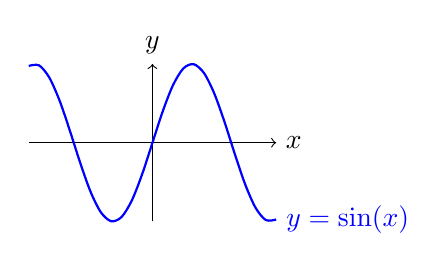
\begin{tikzpicture}
	\draw[->] (-pi/2, 0) -- (pi/2, 0)                                          node[right] {$x$};
	\draw[->] (0, -1) -- (0, 1)                                                node[above] {$y$};
	\draw[blue, thick] [domain=-pi/2:pi/2, smooth] plot (\x, {sin(pi * \x r)}) node[right] {$y = \sin(x)$};
\end{tikzpicture}

\begin{align*}
	S_\text{прямокутника} & = (\frac{\pi}{2} - (-\frac{\pi}{2})) * (1 - 0) = \pi \\
	S_\text{кривої}       & = \int_{-\frac{\pi}{2}}^{\frac{\pi}{2}} \sin(x)dx
	= 2 * \int_{0}^{\frac{\pi}{2}} \sin(x)dx
	= 2 * [-\cos(x)]_{0}^{\frac{\pi}{2}} =                                       \\
	                      & = 2 * (-\cos(\frac{\pi}{2}) + \cos(0))
	= 2 * (0 + 1) = 2                                                            \\
	S_\text{вище кривої}  & = \pi - 2                                            \\
	P                     & = \frac{S_\text{вище кривої}}{S_\text{прямокутника}}
	= \frac{\pi - 2}{\pi} \approx 0.36
\end{align*}

\section{Завдання 32}

В середені прямокутника, обмеженого віссю $OX$,
прямими $x = \frac{\pi}{2}$, $x = -\frac{\pi}{2}$, $y = 1$,
навмання вибрано точку. Знайти ймовірність того,
що точка знаходиться вище лінії $y = cos(x)$.

\subsection*{Розв'язння}

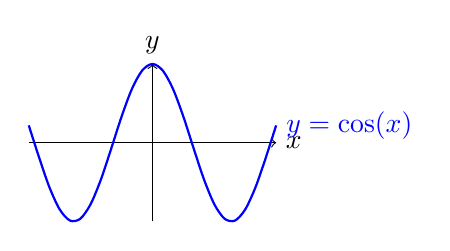
\begin{tikzpicture}
	\draw[->] (-pi/2, 0) -- (pi/2, 0)                                          node[right] {$x$};
	\draw[->] (0, -1) -- (0, 1)                                                node[above] {$y$};
	\draw[blue, thick] [domain=-pi/2:pi/2, smooth] plot (\x, {cos(pi * \x r)}) node[right] {$y = \cos(x)$};
\end{tikzpicture}

\begin{align*}
	S_\text{прямокутника} & = (\frac{\pi}{2} - (-\frac{\pi}{2})) * (1 - 0) = \pi \\
	S_\text{кривої}       & = \int_{-\frac{\pi}{2}}^{\frac{\pi}{2}} \cos(x)dx
	= 2 * \int_{0}^{\frac{\pi}{2}} \cos(x)dx
	= 2 * [\sin(x)]_{0}^{\frac{\pi}{2}} =                                        \\
	                      & = 2 * (\sin(\frac{\pi}{2}) - \sin(0))
	= 2 * (1 - 0) = 2                                                            \\
	S_\text{вище кривої}  & = \pi - 2                                            \\
	P                     & = \frac{S_\text{вище кривої}}{S_\text{прямокутника}}
	= \frac{\pi - 2}{\pi} \approx 0.36
\end{align*}

\end{document}
